\documentclass{beamer}
\usepackage[utf8]{inputenc}
\usepackage{tikz}
\usepackage{algorithm}
\usepackage{algpseudocode}

\usetheme{Antibes}
\usecolortheme{crane}

%------------------------------------------------------------
%This block of code defines the information to appear in the
%Title page
\title[Problema dei Tubi] %optional
{Problema dei Tubi}

\subtitle{A short story}

\author[GR03A] % (optional)
{Luca Mazza \and Vasco Silva Pereira \and Sebastiano Piubellini}


%End of title page configuration block
%------------------------------------------------------------



%------------------------------------------------------------
%The next block of commands puts the table of contents at the 
%beginning of each section and highlights the current section:

\AtBeginSection[]
{
  \begin{frame}
    \frametitle{Table of Contents}
    \tableofcontents[currentsection]
  \end{frame}
}
%------------------------------------------------------------


\begin{document}

%The next statement creates the title page.
\frame{\titlepage}


%---------------------------------------------------------
%This block of code is for the table of contents after
%the title page
\begin{frame}
\frametitle{Table of Contents}
\tableofcontents
\end{frame}
%---------------------------------------------------------


\section{Introduzione}

%---------------------------------------------------------
%Changing visivility of the text
\begin{frame}
\frametitle{Introduzione}
Problema di ottimizzazione di una fabbrica di cioccolato,
manutenzione delle linee di trasporto del cioccolato.

\begin{itemize}
    \item Giunti interconnettono i rami di produzione (\textit{nodes})
    \item Ogni giunto ha un tempo di manutenzione
    \item Giunti di ricambio a disposizione
    \item Cambiando un giunto si azzera
\end{itemize}
\end{frame}

%---------------------------------------------------------


\section{Risoluzione del problema}

%---------------------------------------------------------
%Highlighting text
\begin{frame}
\frametitle{Risoluzione del problema}

Ci siamo basati sul prototipo dell'algoritmo \alert{DFS} 
per sviluppare l'algoritmo.
Fin da subito, abbiamo capito che questo poteva essere 
una possibile soluzione del problema.

\begin{block}{Funzionamento}
DFS esplora un albero, partendo dalla radice, dando 
priorità all'esplorazione in profondità.

\end{block}

\end{frame}
\begin{frame}
\frametitle{Risoluzione del problema}
\begin{center}
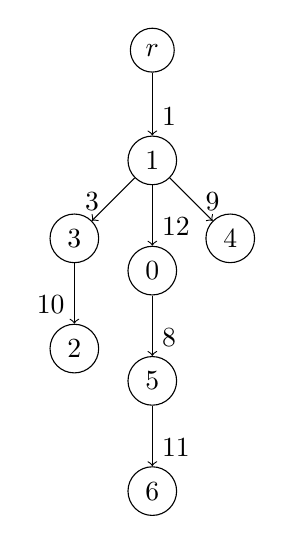
\begin{tikzpicture}[node distance={14mm}, main/.style = {draw, circle}]
\node[main] (-1) {$r$}; 
\node[main] (1) [below of=-1] {$1$}; 
\node[main] (0) [below of=1] {$0$}; 
\node[main] (3) [below left of=1] {$3$}; 
\node[main] (2) [below of=3] {$2$}; 
\node[main] (5) [below of=0] {$5$}; 
\node[main] (6) [below of=5] {$6$}; 
\node[main] (4) [below right of=1] {$4$}; 
\draw[->] (-1) -- node[midway, above right, pos=1] {1} (1);
\draw[->] (1) -- node[midway, above, pos=1] {3} (3);
\draw[->] (3) -- node[midway, above left, pos=1] {10} (2);
\draw[->] (1) -- node[midway, above right, pos=1] {12} (0);
\draw[->] (0) -- node[midway, above right, pos=1] {8} (5);
\draw[->] (5) -- node[midway, above right, pos=1] {11} (6);
\draw[->] (1) -- node[midway, above, pos=1] {9} (4);
\end{tikzpicture} 
\end{center}
\end{frame}

\begin{frame}
\frametitle{Visita in profondità}
\begin{center}
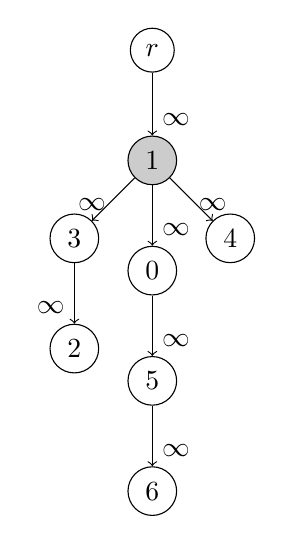
\begin{tikzpicture}[node distance={14mm}, main/.style = {draw, circle}]
\node[main] (-1) [] {$r$}; 
\node[main] (1) [below of=-1,fill=black!20] {$1$}; 
\node[main] (0) [below of=1] {$0$}; 
\node[main] (3) [below left of=1] {$3$}; 
\node[main] (2) [below of=3] {$2$}; 
\node[main] (5) [below of=0] {$5$}; 
\node[main] (6) [below of=5] {$6$}; 
\node[main] (4) [below right of=1] {$4$}; 
\draw[->] (-1) -- node[midway, above right, pos=1] {$\infty$} (1);
\draw[->] (1) -- node[midway, above, pos=1] {$\infty$} (3);
\draw[->] (3) -- node[midway, above left, pos=1] {$\infty$} (2);
\draw[->] (1) -- node[midway, above right, pos=1] {$\infty$} (0);
\draw[->] (0) -- node[midway, above right, pos=1] {$\infty$} (5);
\draw[->] (5) -- node[midway, above right, pos=1] {$\infty$} (6);
\draw[->] (1) -- node[midway, above, pos=1] {$\infty$} (4);
\end{tikzpicture} 
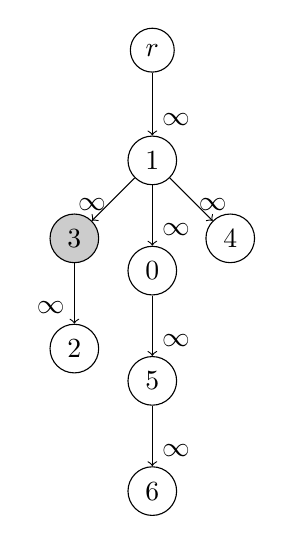
\begin{tikzpicture}[node distance={14mm}, main/.style = {draw, circle}]
\node[main] (-1) [] {$r$}; 
\node[main] (1) [below of=-1] {$1$}; 
\node[main] (0) [below of=1] {$0$}; 
\node[main] (3) [below left of=1,fill=black!20] {$3$}; 
\node[main] (2) [below of=3] {$2$}; 
\node[main] (5) [below of=0] {$5$}; 
\node[main] (6) [below of=5] {$6$}; 
\node[main] (4) [below right of=1] {$4$}; 
\draw[->] (-1) -- node[midway, above right, pos=1] {$\infty$} (1);
\draw[->] (1) -- node[midway, above, pos=1] {$\infty$} (3);
\draw[->] (3) -- node[midway, above left, pos=1] {$\infty$} (2);
\draw[->] (1) -- node[midway, above right, pos=1] {$\infty$} (0);
\draw[->] (0) -- node[midway, above right, pos=1] {$\infty$} (5);
\draw[->] (5) -- node[midway, above right, pos=1] {$\infty$} (6);
\draw[->] (1) -- node[midway, above, pos=1] {$\infty$} (4);
\end{tikzpicture}
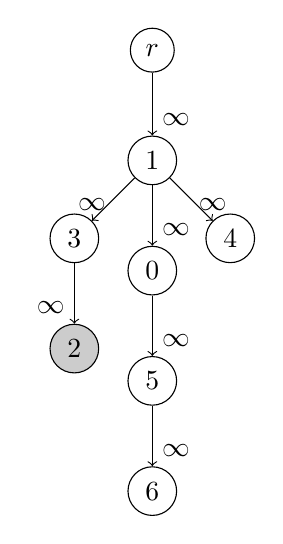
\begin{tikzpicture}[node distance={14mm}, main/.style = {draw, circle}]
\node[main] (-1) [] {$r$}; 
\node[main] (1) [below of=-1] {$1$}; 
\node[main] (0) [below of=1] {$0$}; 
\node[main] (3) [below left of=1] {$3$}; 
\node[main] (2) [below of=3,fill=black!20] {$2$}; 
\node[main] (5) [below of=0] {$5$}; 
\node[main] (6) [below of=5] {$6$}; 
\node[main] (4) [below right of=1] {$4$}; 
\draw[->] (-1) -- node[midway, above right, pos=1] {$\infty$} (1);
\draw[->] (1) -- node[midway, above, pos=1] {$\infty$} (3);
\draw[->] (3) -- node[midway, above left, pos=1] {$\infty$} (2);
\draw[->] (1) -- node[midway, above right, pos=1] {$\infty$} (0);
\draw[->] (0) -- node[midway, above right, pos=1] {$\infty$} (5);
\draw[->] (5) -- node[midway, above right, pos=1] {$\infty$} (6);
\draw[->] (1) -- node[midway, above, pos=1] {$\infty$} (4);
\end{tikzpicture} 
\end{center}
\end{frame}

\begin{frame}
\frametitle{Riavvolgimento}
\begin{center}
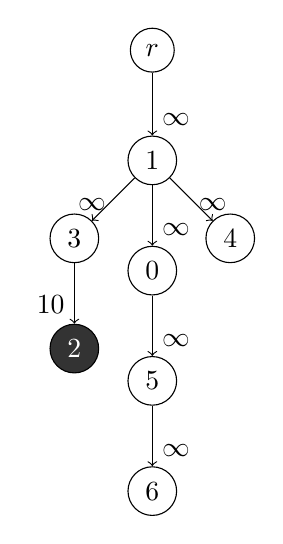
\begin{tikzpicture}[node distance={14mm}, main/.style = {draw, circle}]
\node[main] (-1) [] {$r$}; 
\node[main] (1) [below of=-1] {$1$}; 
\node[main] (0) [below of=1] {$0$}; 
\node[main] (3) [below left of=1] {$3$}; 
\node[main] (2) [below of=3,fill=black!80,text=white] {$2$}; 
\node[main] (5) [below of=0] {$5$}; 
\node[main] (6) [below of=5] {$6$}; 
\node[main] (4) [below right of=1] {$4$}; 
\draw[->] (-1) -- node[midway, above right, pos=1] {$\infty$} (1);
\draw[->] (1) -- node[midway, above, pos=1] {$\infty$} (3);
\draw[->] (3) -- node[midway, above left, pos=1] {$10$} (2);
\draw[->] (1) -- node[midway, above right, pos=1] {$\infty$} (0);
\draw[->] (0) -- node[midway, above right, pos=1] {$\infty$} (5);
\draw[->] (5) -- node[midway, above right, pos=1] {$\infty$} (6);
\draw[->] (1) -- node[midway, above, pos=1] {$\infty$} (4);
\end{tikzpicture}
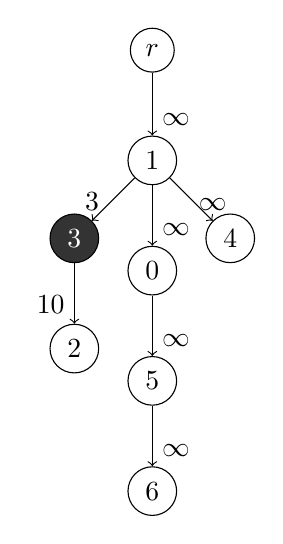
\begin{tikzpicture}[node distance={14mm}, main/.style = {draw, circle}]
\node[main] (-1) [] {$r$}; 
\node[main] (1) [below of=-1] {$1$}; 
\node[main] (0) [below of=1] {$0$}; 
\node[main] (3) [below left of=1,fill=black!80,text=white] {$3$}; 
\node[main] (2) [below of=3] {$2$}; 
\node[main] (5) [below of=0] {$5$}; 
\node[main] (6) [below of=5] {$6$}; 
\node[main] (4) [below right of=1] {$4$}; 
\draw[->] (-1) -- node[midway, above right, pos=1] {$\infty$} (1);
\draw[->] (1) -- node[midway, above, pos=1] {$3$} (3);
\draw[->] (3) -- node[midway, above left, pos=1] {$10$} (2);
\draw[->] (1) -- node[midway, above right, pos=1] {$\infty$} (0);
\draw[->] (0) -- node[midway, above right, pos=1] {$\infty$} (5);
\draw[->] (5) -- node[midway, above right, pos=1] {$\infty$} (6);
\draw[->] (1) -- node[midway, above, pos=1] {$\infty$} (4);
\end{tikzpicture}
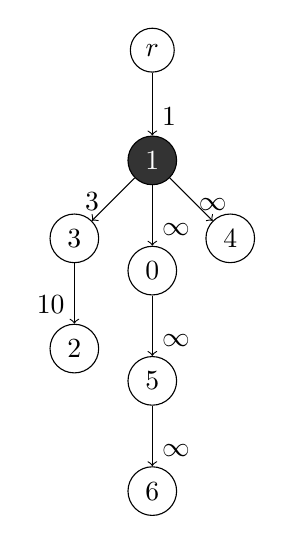
\begin{tikzpicture}[node distance={14mm}, main/.style = {draw, circle}]
\node[main] (-1) [] {$r$}; 
\node[main] (1) [below of=-1,fill=black!80,text=white] {$1$}; 
\node[main] (0) [below of=1] {$0$}; 
\node[main] (3) [below left of=1] {$3$}; 
\node[main] (2) [below of=3] {$2$}; 
\node[main] (5) [below of=0] {$5$}; 
\node[main] (6) [below of=5] {$6$}; 
\node[main] (4) [below right of=1] {$4$}; 
\draw[->] (-1) -- node[midway, above right, pos=1] {$1$} (1);
\draw[->] (1) -- node[midway, above, pos=1] {$3$} (3);
\draw[->] (3) -- node[midway, above left, pos=1] {$10$} (2);
\draw[->] (1) -- node[midway, above right, pos=1] {$\infty$} (0);
\draw[->] (0) -- node[midway, above right, pos=1] {$\infty$} (5);
\draw[->] (5) -- node[midway, above right, pos=1] {$\infty$} (6);
\draw[->] (1) -- node[midway, above, pos=1] {$\infty$} (4);
\end{tikzpicture} 
\end{center}
\end{frame}

\begin{frame}[allowframebreaks]
\frametitle{Pseudocodice}
\small\begin{breakablealgorithm}
\begin{algorithmic}[1]
\Procedure{MinimizeTime}{node}
    \If{$\text{child\_count}[node] = 0$} \Comment{Base case}
        \State $\text{mem}[node][0] \gets T[node]$
        \For{$c \gets 1$ to $C$}
            \State $\text{mem}[node][c] \gets 0$
        \EndFor 
        \State \Return
    \EndIf
    \framebreak
    \For{each child $v$ of $node$ in $\text{adj}[node]$} \Comment{Recursive case}
        \State \Call{MinimizeTime}{$v$}
        \State Initialize $\text{cur}[0 \dots C] \gets \infty$
        \For{$c \gets 0$ to $C$}
            \For{$x \gets 0$ to $c$}
                \State $\text{cur}[c] \gets \min(\text{cur}[c], \max(\text{mem}[v][x], \text{mem}[node][c - x]))$
            \EndFor
        \EndFor
        \State $\text{mem}[node][...] \gets \text{cur}[...]$
    \EndFor
    \State Initialize $\text{cur}[0 \dots C]$
    \State $\text{cur}[0] \gets T[node] + \text{mem}[node][0]$
    \framebreak
    \For{$c \gets 1$ to $C$} \Comment{Wrap-up}
        \State $\text{cur}[c] \gets \min(T[node] + \text{mem}[node][c], \text{mem}[node][c - 1])$
    \EndFor
    \State $\text{mem}[node][...] \gets \text{cur}[...]$
\EndProcedure
\end{algorithmic}
\end{breakablealgorithm}
\end{frame}

\begin{frame}
\frametitle{Risoluzione del problema}

Una volta visitati tutti i nodi l'algoritmo prova, per ogni ricambio, ad applicare $c$ ricambi e $(c - x)$ per il resto del sistema.
Viene poi aggiornato il valore attuale calcolato per $c$ ricambi che minimizza il massimo valore tra:
\begin{itemize}
   \item Il risultato del sottoalbero radicato in $v$ con $x$ ricambi;
   \item Il risultato del nodo corrente e degli altri sottoalberi con $c-x$ ricambi.
\end{itemize}

$$cur(c) = \min(cur(c), \max(S_v(x), S_u(c - x)))$$

\end{frame}
%---------------------------------------------------------

\section{Complessità}

%---------------------------------------------------------
\begin{frame}{Complessità}
    \begin{itemize}
        \item N: giunti da riparare, C: giunti sostituibili
        \item Complessità temporale: \begin{math}O(N * C^2)\end{math}
        \item Complessità spaziale: \begin{math}O(N * C)\end{math}
        \item Dati calcolati da una media di 10 test per ogni task
    \end{itemize}    
\end{frame}

\begin{frame}{Complessità - memoria occupata}
    \begin{columns}
    \begin{column}{0.5\textwidth}
    \begin{figure}
        \includegraphics[width=1\linewidth]{memoria occupata.png}
        \caption{Utilizzo memoria}
    \end{figure}
    \end{column}
     \begin{column}{0.5\textwidth}
            \begin{itemize}
                \item La memoria occupata cresce proporzionalmente a numero giunti (N) e giunti sostituibili (C)
            \end{itemize}
        \end{column}
    \end{columns}
    
\end{frame}

\begin{frame}{Complessità - tempo di esecuzione}
\begin{columns}
    \begin{column}{0.5\textwidth}
     \begin{figure}
        \includegraphics[width=1\linewidth]{tempo cpu.png}
        \caption{Tempo CPU}
    \end{figure}
    \end{column}
     \begin{column}{0.5\textwidth}
            \begin{itemize}
                
            \end{itemize}
        \end{column}
    \end{columns}
\end{frame}

%---------------------------------------------------------

\section{Conclusioni}

%---------------------------------------------------------
%Highlighting text
\begin{frame}
\frametitle{Sample frame title}

In this slide, some important text will be
\alert{highlighted} because it's important.
Please, don't abuse it.

\begin{block}{Remark}
Sample text
\end{block}

\begin{alertblock}{Important }
Sample text in red box
\end{alertblock}

\begin{examples}
Sample text in green box. The title of the block is ``Examples".
\end{examples}
\end{frame}
%---------------------------------------------------------

\end{document}
